\section{Results}
\label{sec:results}

\subsection{The split protocol accounts for most reported performance (\textbf{RQ1})}
\label{sec:ladder}

Table~\ref{tab:ladder} isolates the effect of test partition overlap with training by holding corpus, architecture, node features, folds, and seeds constant.

\begin{table}[h]
\centering
\caption{GAT backbone. All variables except the data
split are held constant: corpus, architecture, node features, folds and seeds
remain unchanged. The \texttt{random} protocol is the standard in existing
literature.}
\label{tab:ladder}
\begin{tabular}{lccc}
\toprule
& \multicolumn{2}{c}{\textbf{ROC-AUC}} & \\
\cmidrule(lr){2-3}
\textbf{Protocol} & \textbf{five-fold} & \textbf{single model} & \textbf{seeds} \\
\midrule
\texttt{random} & $0.796 \pm 0.002$ & $0.774 \pm 0.004$ & 5 \\
\texttt{group}  & $0.657 \pm 0.008$ & $0.702 \pm 0.008$ & 4\rlap{$^\dagger$}/5 \\
\texttt{repo}   & $0.585 \pm 0.012$ & $0.649 \pm 0.012$ & 5 \\
\midrule
leakage share   & $71.5\%$          & $45.5\%$          & \\
\bottomrule
\end{tabular}
\begin{tablenotes}\footnotesize
\item $^\dagger$ One \texttt{group} seed is excluded. It could not be trained at
the batch size used everywhere else, and the reduced-batch rerun is not
comparable: repeating a different seed at that batch size costs $0.059$ ROC-AUC.
\end{tablenotes}
\end{table}

\begin{figure}[h]
\centering
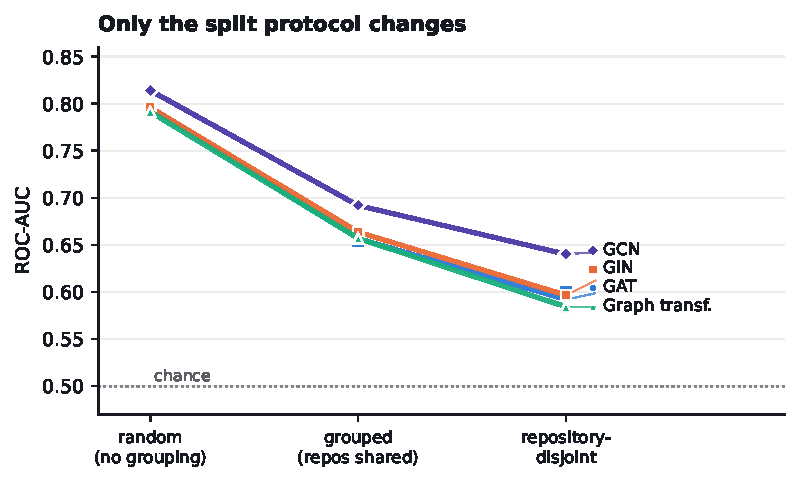
\includegraphics[width=\columnwidth]{ladder.pdf}
\caption{Four graph backbones under the three split protocols. Corpus, node
features, folds and seeds are held fixed; the only thing that varies is what
the test partition is permitted to share with training. All four decline by a
similar amount, and their ordering is broadly preserved, so the effect is a
property of the protocol rather than of any one architecture.}
\label{fig:ladder}
\end{figure}

Figure~\ref{fig:ladder} illustrates the decline across all backbones. Shares
are taken against the margin above chance, not against the raw score: under the
five-fold procedure that margin is $0.796-0.5=0.296$, and the drop to the
repository-disjoint score is $0.796-0.585=0.211$, so
$0.211/0.296 = \textbf{71.5\%}$ of the usable signal is attributable to what the
split permits. Of that margin, \textbf{47.0\%} is due to duplicates, patched
twins and shared commits, \textbf{24.4\%} to repository overlap, and
\textbf{28.5\%} survives every control. The last figure is what remains, not a
further component of the loss.

The second column of Table~\ref{tab:ladder} is the reason this paper reports
two procedures throughout. Holding the corpus, architecture, features and seeds
fixed and changing only whether the reported model is a five-fold ensemble or a
single model trained on the whole partition moves the repository-disjoint score
from $0.585$ to $0.649$ and the leakage share from $71.5\%$ to $45.5\%$. Both
are defensible procedures and neither is stated in the papers we surveyed.
Section~\ref{sec:procedure} examines why they differ.

The $0.796$ ROC-AUC aligns with values commonly reported in the literature, and was achieved without any modifications to the model.

\subsubsection{Replication across architectures}
Table~\ref{tab:arch} extends the analysis to four architectures representing different aggregation mechanisms: attention, spectral convolution, sum aggregation, and global attention as implemented in a graph transformer.

\begin{table}[h]
\centering
\caption{Four architecture families under the repository-disjoint protocol,
five seeds per cell, reported under both training procedures. The ordering of
the architectures differs between the two columns and the spread collapses from
$0.044$ to $0.009$, so architecture comparisons in this setting are not
separable from the training procedure.}
\label{tab:arch}
\begin{tabular}{lccc}
\toprule
\textbf{Backbone} & \textbf{five-fold} & \textbf{single model} & \textbf{difference} \\
\midrule
GAT               & $0.585 \pm 0.012$ & $0.649 \pm 0.012$ & $+0.065$ \\
GCN               & $0.628 \pm 0.008$ & $0.653 \pm 0.008$ & $+0.025$ \\
GIN               & $0.591 \pm 0.009$ & $0.658 \pm 0.015$ & $+0.067$ \\
Graph transformer & $0.587 \pm 0.007$ & $0.650 \pm 0.010$ & $+0.064$ \\
\bottomrule
\end{tabular}
\end{table}

Every architecture gains from the single-model procedure, three of them by
about $0.065$, and all four differences are significant. GCN is the exception at
$+0.025$; we have no account of why and report it as an observation.

Two things in this table bear on how architecture comparisons in this area
should be read. The ordering changes: GCN is strongest under the ensemble and
GIN under the single model. And the spread across four families collapses from
$0.044$ to $0.009$, which is within the seed standard deviation of the
individual cells. Under the better procedure these architectures are not
distinguishable from one another, so a comparison between them is reporting the
training procedure at least as much as the aggregation scheme. GIN is a useful
case: it is the most expressive of the four under the 1-Weisfeiler-Lehman
criterion, unlike GCN and GAT, and it is third of four under one procedure and
nominally first under the other, by a margin smaller than noise. This motivates
the analysis in Section~\ref{sec:graph-worth}.

\subsection{The encoding sets what the graph is measured to be worth (\textbf{RQ2})}
\label{sec:graph-worth}

The protocol above fixes what is being measured. Within it we vary how the
graph is presented to the network, holding the corpus, the architecture, the
node features and the training schedule constant. Two encoding choices are
available and neither is varied in this literature. One of them changes the
measured contribution of the graph by more than most published architectural
improvements; the other changes nothing at all. Which is which is not
predictable from how meaningful the choice sounds.

\subsubsection{Edge relation types}
Joern labels each edge with the relation it represents: abstract syntax, control
flow, data dependence or control dependence. Collapsing those four labels into a
single undifferentiated relation, while leaving the connectivity untouched,
isolates what the labels are worth.

The comparison must hold edge direction fixed. Because reversed edges are
encoded as additional relation types (Section~\ref{sec:method}), collapsing the
labels in a directed graph and in a bidirectional one are different
interventions, and an unmatched pair confounds the two. Both arms below are
bidirectional; connectivity is identical, and only the distinguishability of the
four relations varies.

\begin{table}[h]
\centering
\caption{Effect of relation labels, five seeds per cell, repository-disjoint.
Both arms bidirectional, so direction is held fixed and only the four relation
labels vary. Seed standard deviations are $0.005$--$0.012$ throughout; the GIN
row is discussed below.}
\label{tab:typed}
\small
\begin{tabular}{lcccc}
\toprule
\textbf{Backbone} & \textbf{typed} & \textbf{collapsed} & \textbf{effect} & \textbf{95\% CI} \\
\midrule
GAT         & $0.618$ & $0.620$ & $-0.002$ & $[-0.012,+0.007]$ \\
GCN         & $0.634$ & $0.624$ & $+0.010$ & $[-0.007,+0.026]$ \\
G.\ transf. & $0.603$ & $0.603$ & $-0.001$ & $[-0.022,+0.021]$ \\
\midrule
GIN$^\dagger$ & $0.583$ & $0.589$ & $-0.006$ & $[-0.015,+0.004]$ \\
\bottomrule
\end{tabular}
\begin{tablenotes}\footnotesize
\item $^\dagger$ Cannot read relation labels; true effect is zero by
construction.
\end{tablenotes}
\end{table}

\noindent Pooled over the three architectures whose operators condition on
relation type, distinguishing data dependence from syntactic containment is
worth $+0.002$ ROC-AUC (95\% CI $-0.005$ to $+0.010$, $n=15$). An equivalence
test against a margin of $0.033$, the size of the edge-direction effect below,
rejects an effect of that magnitude at $p<10^{-6}$. The labels are not merely
unproven here; they are bounded to within a third of the run-to-run standard
deviation.

The GIN row establishes what that bound means. Its operator sums over
neighbours with no edge-feature term, so the typed and collapsed conditions are
the same model and the true difference is exactly zero. It nonetheless measures
$-0.006$, with individual seeds ranging from $+0.006$ to $-0.012$, which is the
floor imposed by nondeterministic accumulation in scatter operations. No
architecture departs from that floor.

This is the one place where an unmatched comparison would have produced a
different answer. Against a \emph{directed} collapsed baseline the same typed
model appears to gain $+0.024$, but that figure is the edge-direction effect of
Section~\ref{sec:direction} arriving through the relation table, not a property
of the labels.

\begin{figure}[htb]
\centering
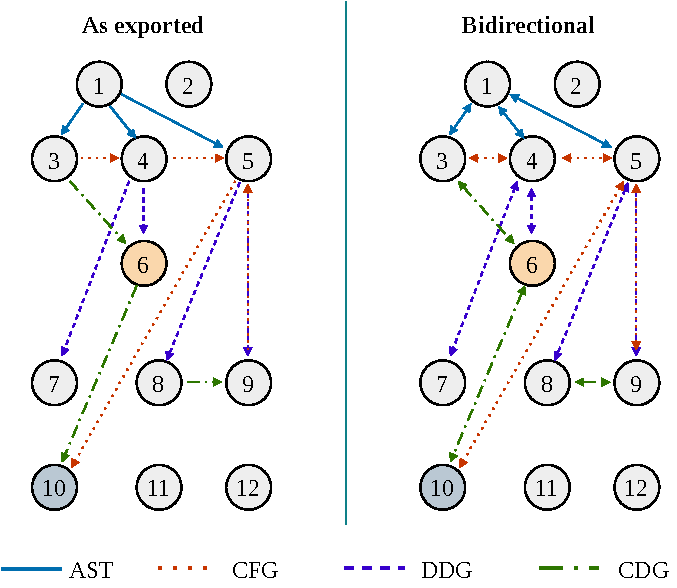
\includegraphics[width=0.85\textwidth]{direct.pdf}
\caption{The same code property graph under both encodings. Edge styles
distinguish the four relations. On the left the edges run in the direction the
exporter emits them, so a node aggregates only from its predecessors. On the
right each edge is additionally traversable in reverse, entered as a distinct
relation type rather than by making the graph undirected, so an operator that
reads the relation label can still tell a forward traversal from a backward
one.}
\label{fig:direction}
\end{figure}

\subsubsection{Edge direction}
\label{sec:direction}
Joern exports the code property graph as a directed object, and the pipeline
above consumes it unaltered. Figure~\ref{fig:direction} contrasts the two
encodings on one graph. A node therefore aggregates only from its
predecessors: an abstract-syntax parent never receives from its children, and a
definition never receives from its uses. Measured over 767 graphs, the average
node reaches only $18.9\%$ of its own function within three layers under this
convention, against $73.8\%$ once each edge is also traversable in the opposite
direction. Widening the receptive field by adding layers instead would incur the
costs this narrows away from~\citep{li2018deeper,alon2021bottleneck}.

Adding every edge back as a distinct reversed relation, which leaves the
parameter count unchanged because the relation table already had unused
capacity, changes the picture materially:

\begin{center}
\small
\begin{tabular}{lccc}
\toprule
\textbf{Protocol} & \textbf{directed} & \textbf{bidirectional} & \textbf{gain ($p$)} \\
\midrule
\texttt{random} & $0.796$ & $0.793$ & $-0.003$ (0.014) \\
\texttt{group}  & $0.657$ & $0.666$ & $+0.009$ (0.286) \\
\texttt{repo}   & $0.585$ & $0.618$ & $+0.033$ (0.012) \\
\bottomrule
\end{tabular}
\end{center}

\noindent All $p$-values are paired $t$-tests over five seeds, the seed being
the unit of replication. The five folds inside a run share a training partition
and a seed and are not independent, so pooling them would inflate the sample
fivefold.

The gain appears only as the protocol tightens. Under \texttt{random}
the reverse direction is slightly harmful, under \texttt{group} it does not
reach significance, and under repository-disjoint evaluation it is worth
$+0.033$ ($p=0.012$). That ordering is consistent with the rest of this section: when
duplicates and patched twins are available, token content alone suffices and
improved structural reach adds nothing. The change is measurable precisely where
generalisation is.

The benefit tracks whether the operator can read the relation label, and it
does so exactly. Repeated at five seeds under the repository-disjoint protocol:

\begin{center}
\small
\begin{tabular}{lcccc}
\toprule
& \textbf{directed} & \textbf{bidirectional} & \textbf{gain} & \textbf{$p$} \\
\midrule
GAT         & $0.585$ & $0.618$ & $+0.033$ & 0.012 \\
G.\ transf. & $0.587$ & $0.603$ & $+0.016$ & 0.010 \\
GCN         & $0.628$ & $0.634$ & $+0.006$ & 0.062 \\
\midrule
GIN         & $0.591$ & $0.583$ & $-0.008$ & 0.043 \\
\bottomrule
\end{tabular}
\end{center}

\noindent Two of the three operators that condition on edge type gain
significantly, GAT by $0.033$ and the graph transformer by $0.016$. GCN gains
$0.006$ at $p=0.062$, which does not establish an effect and we do not count it
as one. GIN, the only operator that cannot read the relation label, is the sole
architecture significantly harmed. The mechanism is direct.
Reversed edges enter as distinct relation types, so an operator that reads the
relation gains the ability to tell a forward traversal from a backward one,
while GIN sums over neighbours with no edge-feature term and receives only a
doubled adjacency it cannot distinguish from the forward graph. We verified
this by relabelling the edge types of a fixed graph, which leaves GIN's output
bit-identical while changing the output of the other three.

This result does not survive a change of training procedure, and that is the
most important thing about it. Repeating the same comparison with a single
model trained on the whole partition, five seeds on each side:

\begin{center}
\small
\small
\begin{tabular}{lcccc}
\toprule
\textbf{Procedure} & \textbf{directed} & \textbf{bidir.} & \textbf{gain} & \textbf{$p$} \\
\midrule
five-fold ensemble & $0.585$ & $0.618$ & $+0.033$ & 0.012 \\
single model       & $0.649$ & $0.643$ & $-0.006$ & 0.41 \\
\bottomrule
\end{tabular}
\end{center}

\noindent The direction of the edges is worth a third of a standard deviation
of nothing once the model is trained the better way, and the better way is also
the stronger one: the worst single-model configuration here exceeds the best
five-fold configuration. The reading we take is not that edge direction is
useless, nor that it is valuable, but that its measured value is contingent on
a choice that no paper in this area reports. An ablation of this kind cannot be
interpreted without the training procedure stated alongside it.

A plausible mechanism ties the two together. The five-fold ensemble's reach
over the graph is limited by what each member learns from four fifths of the
data with an epoch chosen on repositories it has already seen; widening the
receptive field compensates for part of that. A single model trained on the
whole partition does not need the compensation. We do not test this directly
and offer it as an interpretation rather than a result.

\subsubsection{Removing node text}
With text zeroed, leaving node types and graph structure, ROC-AUC is:

\begin{center}
\begin{tabular}{lcc}
\toprule
& \multicolumn{2}{c}{\textbf{ROC-AUC}} \\
\cmidrule(lr){2-3}
& \texttt{random} & \texttt{repo} \\
\midrule
\texttt{type-only} (no text) & 0.714 & 0.476 \\
\texttt{topology} (shape only) & 0.452 & 0.494 \\
\bottomrule
\end{tabular}
\end{center}

Node types alone do not indicate vulnerabilities; for example, the presence of three \texttt{CALL} nodes and two \texttt{IDENTIFIER}s does not reveal a buffer overflow. However, they serve as structural fingerprints. The $0.714$ ROC-AUC under a random split reflects recognition of previously encountered structures rather than true vulnerability detection, and this value surpasses those reported by several published systems. In contrast, under a repository-disjoint split, the same model performs at chance. The \texttt{topology} result establishes the baseline and eliminates function length as a confounding factor, as the MCC is exactly $0.000$.

\begin{figure}[htb]
\centering
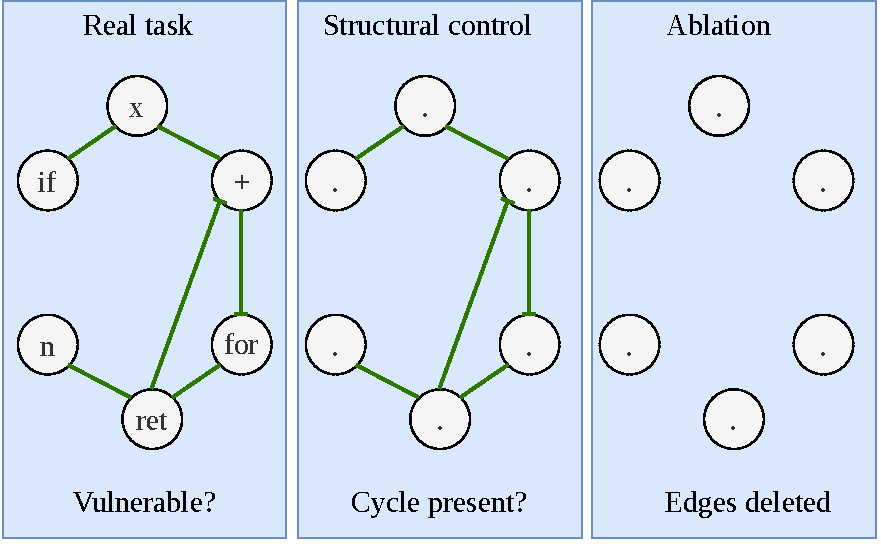
\includegraphics[width=\textwidth]{control.pdf}
\caption{The positive control. Left: the real task, with node text and the
vulnerability label. Centre: the same graphs with node content replaced by
noise and node types collapsed, labelled by a property computable from the edge
set alone. Right: the same again with the edges deleted, which leaves only
graph size. The evidence is the gap between the centre and right conditions.}
\label{fig:control}
\end{figure}

\subsubsection{A positive control for structural learning}
The \texttt{topology} row above is open to two readings. It may mean that graph
shape carries no vulnerability signal, or it may mean that this pipeline cannot
read graph shape at all. Those are competing explanations for the same number,
and the ablations reported so far do not separate them.

The following control does, and Figure~\ref{fig:control} sets out its three
conditions. The graphs are the same real code property graphs, but every node
feature is replaced with random noise and every node type is collapsed to a
single identifier, so nothing about a node carries information.
The labels are chosen to be computable from the edge set alone, which places
them within what message passing of this family can in principle
express~\citep{xu2018how,morris2019weisfeiler}.
The label is then computed from the edge set alone: whether the control-flow
subgraph contains a directed cycle, and whether data-dependence edges outnumber
control-flow edges. A model that can read structure must exceed chance; a model
with the edges deleted retains only the node count.

\begin{center}
\small
\begin{tabular}{lccc}
\toprule
\textbf{Structural label} & \textbf{graph} & \textbf{no graph} & \textbf{gain} \\
\midrule
CFG contains a cycle     & $0.860$ & $0.756$ & $+0.104$ \\
DDG edges $>$ CFG edges  & $0.976$ & $0.673$ & $+0.303$ \\
\bottomrule
\end{tabular}
\end{center}

\noindent Three seeds each. The evidence here is the \emph{gain}, not the
absolute score, and the distinction matters because the edge-free column is far
above chance: $0.756$ for loop presence and $0.673$ for the edge-type ratio.
Both labels are therefore substantially predictable from graph size alone, which
pooling exposes and which both columns share equally. Nothing about the $0.860$
should be read as evidence that the model has understood control flow.

What the comparison does establish is that deleting the edges costs the model
something on a label defined by the edges, $+0.104$ and $+0.303$ on the same
graphs with the same architecture. The second of these is the stronger
instrument: an edge-type ratio is less predictable from node count than loop
presence is, and the gain is three times larger. A pipeline that could not read
the edge set at all would show no gain on either.

Two limits are worth stating. Loop presence and edge-type ratios are coarse,
global properties, and success on them does not establish that the model could
localise a subtle dependency change. And the control shows that the apparatus
can extract edge information, not that the vulnerability label depends on edge
information; those are different claims and only the first is tested here.

\subsection{What the graph representation captures (\textbf{RQ3})}
\label{sec:mechanism}

The encoding choices above recover a contribution of the same order as the
pretrained encoder, and the natural next question is what that recovered signal
consists of. This section asks what the network is doing with the graph it is
given, by
instrumenting a trained model rather than by running further ablations. The
question is not whether the graph helps, which
Section~\ref{sec:graph-worth} measures, but which capabilities the resulting
representation does and does not support.

Deleting the edge set from a trained model at inference, leaving its weights
untouched, isolates the contribution message passing makes to the representation
the classifier consumes. This is instrumentation, not an ablation: no model is
retrained, and the comparison is between two forward passes of the same
network.

Fix a trained GAT and write
\[
  z_G = \operatorname{pool}\bigl(\mathrm{GNN}(X, E)\bigr), \qquad
  z_0 = \operatorname{pool}\bigl(\mathrm{GNN}(X, \varnothing)\bigr)
\]
for the pooled representation the classifier consumes, computed with the real edge set and with the edges deleted under \emph{identical weights}. We report both split protocols; each uses its own independently trained model.

\subsubsection{The network is not over-smoothed}
The standard mechanical explanation for a graph network behaving like a graph-free one is over-smoothing: repeated aggregation acts as a low-pass filter, node representations converge toward a common direction, and any permutation-invariant readout then returns approximately that direction. The diagnostic is the Dirichlet energy over $ L_2$-normalized rows,
\[
E(H) ;=; \frac{1}{|E|}\sum_{(i,j) \in E}
\Bigl| \tfrac{h_i}{|h_i|} - \tfrac{h_j}{|h_j|} \Bigr|^2 ,
\]
which vanishes exactly when message passing has collapsed the representation.

\begin{center}
\begin{tabular}{lcccc}
\toprule
& \multicolumn{2}{c}{\texttt{repo}} & \multicolumn{2}{c}{\texttt{random}} \\
\cmidrule(lr){2-3}\cmidrule(lr){4-5}
& $E(H)$ & pairwise $\cos$ & $E(H)$ & pairwise $\cos$ \\
\midrule
input & $1.342$ & $0.236$ & $1.350$ & $0.231$ \\
GAT 1 & $1.002$ & $0.208$ & $1.038$ & $0.202$ \\
GAT 2 & $0.794$ & $0.246$ & $0.857$ & $0.215$ \\
GAT 3 & $0.643$ & $0.281$ & $0.667$ & $0.266$ \\
\bottomrule
\end{tabular}
\end{center}

Energy decreases by factors of $2.09$ and $2.03$ across the two protocols, but does not approach zero. The mean pairwise cosine similarity between node representations remains between $0.20$ and $0.29$ throughout, decreasing at the first layer and then increasing, ending only $0.045$ and $0.035$ above the initial value for each protocol. These values are far from the near-unity similarity that would indicate collapse. With three layers and median test graph sizes of $75$ and $49$ nodes, the network is not in a collapsed regime. \textbf{Over-smoothing does not account for the observed results}, and neither reducing network depth nor adopting a differentiated propagation scheme would recover the missing performance. All reported quantities are measured on a single trained network per protocol over the entire test partition.

\subsubsection{The edges are used, not ignored}
The network also does not ignore the graph structure. Removing edges from the trained model results in a substantial change in the pooled representation: the mean $\cos(z_G, z_0)$ is $0.726$ for \texttt{repo} and $0.574$ for \texttt{random}, with only $1.4\%$ and $2.4\%$ of graphs, respectively, exceeding $0.99$. This indicates that message passing significantly alters the representation.

How much of that work is new? Fitting a ridge map $W$ on the training partition and decomposing the test representation as $z_G = W z_0 + r$ separates the part recoverable from the edge-free features from the part that is not. The map attains $R^2 = 0.719$ and $0.683$, so roughly $70\%$ of the graph representation
is a linear re-encoding of information already present in the pooled node features. The residual component is substantial: $|r| / |z_G|$ equals $0.4475$ and $0.4506$. The close agreement between the two protocols and the two independently trained models (within $0.004$) suggests that this value reflects the inherent geometry of message passing on these graphs, rather than being an artifact of a particular run.

\subsubsection{What the transformation is worth}
Whether that new component carries anything the classifier can use is a conditional question, and $r$ cannot answer it directly: subtracting a ridge fit removes linear predictability from $z_0$ rather than information, so a probe on $r$ alone conflates novelty with re-encoding. Holding the probe class fixed, we compare instead what each representation supports: $\Delta = \text{ROC-AUC}(z_G) - \text{ROC-AUC}(z_0)$.

\begin{center}
\begin{tabular}{lccc}
\toprule
& $z_0$ & $z_G$ & $\Delta$ \\
\midrule
\multicolumn{4}{l}{\emph{\texttt{repo}}} \\
linear             & $0.5814$ & $0.5991$ & $+0.018$ \\
MLP                & $0.5792$ & $0.5780$ & $-0.001$ \\
gradient boosting  & $0.5750$ & $0.6020$ & $+0.027$ \\
\midrule
\multicolumn{4}{l}{\emph{\texttt{random}}} \\
linear             & $0.7698$ & $0.7793$ & $+0.010$ \\
MLP                & $0.7783$ & $0.7783$ & $-0.000$ \\
gradient boosting  & $0.7804$ & $0.7953$ & $+0.015$ \\
\bottomrule
\end{tabular}
\end{center}

The MLP results should not be interpreted as null findings: the seed standard deviation for $z_G$ is $0.006$ and $0.011$, placing $\Delta$ within the range of measurement noise. Additionally, on \texttt{repo}, the MLP does not match the performance of a linear probe on the same input. Gradient boosting provides more stable results, with seed standard deviations between $0.0007$ and $0.0028$, and yields positive values under both protocols. Selecting the best probe for each representation results in $+0.021$ on \texttt{repo} and $+0.015$ on \texttt{random}.

The graph therefore contributes information that is not recoverable from the node features alone. This estimate is independent of the end-to-end ablation of Section~\ref{sec:graph-worth}, which retrains from scratch rather than probing a fixed representation. On \texttt{repo}, the two are close, $+0.014$ retrained against $+0.021$ probed; on \texttt{random}, they are not, $+0.003$ against $+0.015$.

The probe results should be interpreted as upper bounds. In this context, $z_0$ is not derived from a properly trained graph-free model; rather, it is obtained by removing edges at inference from a network trained with edge information, resulting in weights adapted to inputs that are no longer present. This mismatch artificially inflates $\Delta$ relative to a fair comparison in which a graph-free model is trained independently. The retrained ablation provides a more accurate measurement, while the probe quantifies the maximum potential contribution of the graph.

\subsubsection{Discrimination within vulnerable/patched pairs}
A natural objection to the aggregate figures is that they average over easy
cases. Swapping two statements can alter control or data flow while leaving the
node set almost unchanged, and such a case must depend on structure; a test
partition dominated by unrelated safe functions would hide it. We therefore
evaluate on the $2{,}067$ vulnerable/patched pairs held entirely within the test
partition, scoring a model correct when it ranks the vulnerable member above its
own patched twin. Project identity, length and style cancel within a pair. Pairs
are split by whether node text is near-identical (Jaccard $\geq 0.95$), which
isolates the cases where structure is the only difference.

\begin{center}
\begin{tabular}{lccc}
\toprule
\textbf{Slice} & \textbf{pairs} & \textbf{graph} & \textbf{no graph} \\
\midrule
structure only & $165$  & $0.502$ & $0.388$ \\
text differs   & $1{,}341$ & $0.469$ & $0.467$ \\
\bottomrule
\end{tabular}
\end{center}

\noindent Five seeds. The graph is worth $+0.114$ ($p=0.038$) on the
structure-only slice and nothing at all where text also differs ($+0.001$,
$p=0.98$), and the contrast between the two slices is itself significant
($p=0.024$). The aggregate metric does dilute a real, slice-specific effect.

The absolute values matter more than the difference. On the structure-only
slice the graph model reaches $0.502$, which is chance, while the edge-free
model is anti-correlated at $0.388$. Adding edges removes a systematic error
rather than conferring skill. Repeating the measurement with the bidirectional
encoding of Section~\ref{sec:graph-worth} leaves this unchanged: $0.497 \pm
0.033$ against $0.502 \pm 0.057$ over the same five seeds ($p=0.85$), and the
bidirectional model is itself indistinguishable from chance ($p=0.85$ against
$0.5$). The encoding that recovers the largest aggregate gain in this paper
recovers nothing here. \textbf{No configuration we tested distinguishes a
vulnerable function from its own patch at better than chance}, which is
consistent with the paired evaluation of PrimeVul~\citep{ding2024primevul} and
is the sharper form of this paper's claim.

\subsubsection{Reading}
Three properties of the trained model fit together. It is not over-smoothed, it
does use its edges, and message passing induces a large geometric change in the
pooled representation. Yet on the discrimination that matters, separating a
function from its own patch, no configuration exceeds chance.

The encoding results of Section~\ref{sec:graph-worth} are therefore real, and
bounded in a specific way. Restoring edge direction and preserving relation
labels each recover aggregate ROC-AUC, and the instrumentation here indicates
what that recovered signal does and does not support: the representation the network builds from the graph
separates vulnerable from safe functions in aggregate, without localising the
defect that distinguishes a function from its fix.

We are explicit about what this does not establish. It does not show that code
property graphs cannot support that capability, only that this pipeline's
representation does not. One plausible account is that a function-level graph
omits the interprocedural flow many real vulnerabilities depend on, so the
structure available at this scope is thin; testing that requires a different
experiment than the ones reported here, and we do not claim it.

\subsection{Calibrating the protocol against a published model (\textbf{RQ4})}
\label{sec:linevul}

Every measurement so far is internal to one pipeline, which leaves one
alternative explanation open: that the repository-disjoint partition is simply
too hard, or the corpus too noisy, for any model to do well on. If that were so,
the encoding effects reported above would be differences between degrees of
failure rather than measurements of anything. An external model settles it.
LineVul~\citep{fu2022linevul} is a published token-based detector that fine-tunes
CodeBERT on raw function text and uses no graph. We ran the authors'
implementation unmodified, adding only a prediction-score dump, on the identical
splits. Table~\ref{tab:linevul} reports the result.

\begin{table}[h]
\centering
\caption{Official LineVul (authors' code) on the same splits and the same test
partitions as our graph models. Seed coverage as in Table~\ref{tab:arch}: the
\texttt{repo} column and the leakage share are five-seed means, the other
columns single runs except for GAT. The purpose is to establish that the
repository-disjoint partition carries learnable signal, and to compare how much
of each model's performance depends on the protocol.}
\label{tab:linevul}
\begin{tabular}{lcccc}
\toprule
& \multicolumn{3}{c}{\textbf{ROC-AUC}} & \textbf{leakage} \\
\cmidrule(lr){2-4}
& \texttt{random} & \texttt{group} & \texttt{repo} & \\
\midrule
GAT (graph)          & 0.796 & 0.657 & 0.585 & 71.4\% \\
GCN (graph)          & 0.814 & 0.692 & 0.628 & 59.2\% \\
GIN (graph)          & 0.796 & 0.664 & 0.591 & 69.3\% \\
\textbf{LineVul (no graph)} & \textbf{0.914} & \textbf{0.856} & \textbf{0.792} & \textbf{29.5\%} \\
\bottomrule
\end{tabular}
\end{table}

\noindent The first thing this establishes is that the partition is not
degenerate. A published model reaches $0.792$ ROC-AUC on the same
repository-disjoint test functions, so the corpus and the split carry signal
that a learner can find, and the lower figures reported above are properties of
what was measured rather than of an unlearnable task.

The second is a difference in how much each model depends on the protocol.
Only $29.5\%$ of LineVul's signal above chance is attributable to leakage,
against $59.2$--$71.4\%$ for the graph models; its decomposition is $14.1\%$
duplicates and twins, $15.4\%$ repository overlap, and $70.5\%$ surviving every
control. The ranking of the two approaches under a permissive protocol is
therefore a poor guide to their ranking under a strict one.

We report this as calibration and not as a verdict, for two reasons. LineVul
fine-tunes its encoder end to end while the graph models here consume frozen
features, so any absolute difference mixes representation with training regime
(Section~\ref{sec:threats}). And the published graph detectors were not run, so
nothing here bounds what a different graph pipeline could achieve; what
Section~\ref{sec:graph-worth} shows is that at least one encoding choice in our
own was leaving signal unused.

\subsubsection{Training procedure}
\label{sec:procedure}
Everything above is reported under one training configuration: a five-fold
ensemble, each member trained on four fifths of the training partition with the
library defaults inherited from the stage-1 pipeline. That configuration is a
choice, and this section measures what the choice is worth. It is the largest
effect in this paper.

Two factors are confounded in any naive comparison and we separate them. The
first is \emph{ensembling}: five models on four fifths each, averaged, against
one model on the whole partition. The second is the \emph{recipe}: the epoch
budget, effective batch size, learning rate and schedule. Holding the recipe
fixed and varying only the first gives a $2\times2$ with five seeds per cell:

\begin{table}[h]
\centering
\caption{Ensembling and recipe, separated. All cells are GAT, bidirectional,
repository-disjoint, five seeds, selecting the epoch on the same held-out
validation partition. The default recipe is the stage-1 inheritance (120
epochs, batch 256, plateau decay); the selected recipe is described below.}
\label{tab:procedure}
\small
\begin{tabular}{lcc}
\toprule
& \textbf{default recipe} & \textbf{selected recipe} \\
\midrule
one model, whole partition & $0.585 \pm 0.018$ & $0.650 \pm 0.004$ \\
five-fold ensemble         & $0.618 \pm 0.010$ & $0.649 \pm 0.004$ \\
\bottomrule
\end{tabular}
\end{table}

\noindent Three things follow. Ensembling is worth $+0.033$ ($p=0.007$) under
the default recipe and $-0.002$ ($p=0.59$) under the selected one, so it is not
a property of the method but a compensation for undertrained members. The extra
fifth of training data is worth $+0.003$ ($p=0.73$) and can be set aside. And
the recipe is worth $+0.032$ ($p=0.0001$) measured between the best cell
available under each, which is larger than any representational effect reported
in this paper.

\paragraph{How the recipe was selected.} A comparison of two recipes is only
evidence if neither was chosen on the test set. We therefore fixed the
alternative by grid search on the validation partition alone: epoch budget
$\{15, 30\}$, effective batch $\{128, 256\}$, learning rate
$\{10^{-3}, 5\times10^{-4}, 2\times10^{-4}\}$, twelve configurations, ranked by
validation ROC-AUC with the test partition untouched until the ranking was
fixed. The selected configuration is 30 epochs, effective batch 128, learning
rate $2\times10^{-4}$, re-run at five seeds for the figure above.

That search carries its own finding. Across the twelve configurations,
validation ROC-AUC spans $0.015$ while test spans $0.029$, and the rank
correlation between them is weak ($\rho=0.32$, $p=0.31$). Selecting on
validation returns a test score of $0.650$; the best test score in the grid is
$0.661$, at a configuration ranked seventh on validation. Honest selection
therefore leaves roughly a point of ROC-AUC unreachable, and a reported figure
near the top of that range is more likely to reflect selection on test than a
better method. We note the limitation that the grid uses one seed per cell, and
the seed standard deviation at this protocol is about a third of the test range
it spans, so the spread should be read as an upper bound on recipe sensitivity
rather than a point estimate.

\subsection{Absolute performance}
At a 1\% false-positive rate, the graph pipeline's recall under the
repository-disjoint protocol is \textbf{$0.016$}: it finds about two of every
hundred vulnerable functions at an alert volume a reviewer would tolerate. On
the identical test partition, LineVul's recall at the same false-positive rate
is \textbf{$0.278$}, seventeen times higher. Aggregate figures for the graph
pipeline are ROC-AUC $0.585 \pm 0.012$ and MCC $0.061 \pm 0.008$. For ten-way CWE-family classification, macro-F1 is $0.093$, below the $0.100$ chance baseline, indicating performance worse than random guessing. During training, validation macro-F1 reaches $0.65$, but drops to $0.40$ on the test set, suggesting the model memorizes training repositories and fails to generalize.

These figures pertain to the graph-based pipeline, not to vulnerability
detection as a whole. On the same corpus and the same repository-disjoint
partition, LineVul reaches ROC-AUC $0.792$ and MCC $0.438$
(Section~\ref{sec:linevul}), against $0.658$ for the strongest graph
configuration we measured, a single-model GIN. The comparison is not
like-for-like in one respect that should be stated plainly: LineVul fine-tunes
CodeBERT end to end, while every graph model here keeps GraphCodeBERT frozen. A strict protocol does not cost every method equally: the token model
retains most of its performance where this pipeline does not. That ordering is consistent with reports that pretrained token models remain competitive with structure-aware ones once evaluation is tightened~\citep{steenhoek2023empiricalstudydeeplearning,li2025revisitingpretrainedlanguagemodels}.

\subsection{Run-to-run variance}
\label{sec:variance-result}
Run-to-run standard deviation is approximately $0.010$ under the \texttt{repo} protocol ($0.011$ with the graph, $0.010$ without), which is comparable to the effect sizes under investigation~\citep{arcuri2011practical,errica2020fair}. The standard deviation is lower under the \texttt{random} protocol ($0.002$), indicating that variability is greatest under the more rigorous protocol. Single-seed measurements in this study proved unreliable in
both directions:

\begin{center}
\begin{tabular}{lccc}
\toprule
\textbf{Contribution (ROC-AUC)} & $n{=}1$ & $n{=}3$ & $n{=}5$ \\
\midrule
GraphCodeBERT, \texttt{repo} & $-0.022$ & $-0.003$ & $-0.001$ \\
bag-of-words, \texttt{repo}  & $+0.024$ & $+0.023$ & $+0.013$ \\
edge types, \texttt{repo}    & $-0.021$ & $-0.011$ & $-0.009$ \\
\bottomrule
\end{tabular}
\end{center}

The first estimate shrinks by a factor of twenty-eight as seeds accumulate; the other two roughly halve. Individual seeds also disagree with the five-seed mean in sign in every row, and in the first row three of the five do. A single run therefore fixes neither the magnitude nor the direction of these effects. Seed counts are reported throughout, and single-run ablations in this literature should be regarded as provisional.

